\chapter{Theoretical framework}
\label{sec:theory}
\section{The Standard Model of particle physics}
The Standard Model (SM) of particle physics is a renormalizable quantum field theory based on gauge invariance principles.
The underlying principle is the quantization of the elementary constituents of matter and force carriers,
as excitations of the corresponding quantum fields.
At its core, the Standard Model postulates a set of elementary particles, divided into fermions, with half-integer spin and bosons, with integer spin.
It describes three of the four known fundamental interactions: electromagnetism, the weak nuclear force, and the strong nuclear force.

The fundamental interactions obey a local gauge symmetry, which is associated to a Lie group $U(1)_Y \otimes SU(2)_T \otimes SU(3)_C$,
where Y, T and C denote the quantum numbers hypercharge, weak isospin and colour.

The interactions are mediated by gauge bosons such as the photon, the W and Z bosons and the gluons.
The strong interaction is governed by quantum chromodynamics (QCD), a gauge field theory based on colour symmetry group $SU(3)_C$,
and its eight generators correspond to the gluons.
The electroweak interaction is described by a gauge field theory that is invariant under both weak isospin $T_3$ and hypercharge $Y$,
corresponding to the group $U(1)_Y$ $\otimes SU(2)_T$;
the electroweak interaction encompasses both electromagnetic and weak nuclear interactions,
mediated by the photon and by the \PWp, \PWm and \PZz boson respectively,
which come from the mixing of the generators of the two groups
occurring due to the electroweak symmetry breaking,
as explained later in Section~\ref{EWSB}.
The fundamental bosons all have spin 1, except for the Higgs Boson, which is the only known fundamental particle in the theory with spin 0.

Matter is described in the SM by twelve fermion fields.
All of the fundamental fermions have spin $\frac{1}{2}$ and include quarks, which constitute protons and neutrons, as well as leptons like electrons and neutrinos.
Quarks and leptons are further divided into three generations, each with two particles with different weak isospin, for a total of twelve elementary particles, as detailed in Table \ref{tab:fermions}; each fermion has a corresponding antiparticle with the same mass and spin and opposite charges for the three gauge groups.
Fermions belonging to different generations have been observed to have different masses, which are not predicted by the model and must be determined experimentally.

Quarks have colour charge, anti-quarks carry anti-colour, while leptons have no net colour charge, which is called ``white'' colour.
%% Free particles must have a net colour charge of zero due to colour confinement, which is a property of the strong interaction.
Gluons carry both a colour and an anti-colour charge, while all the other fundamental bosons, as well as bound states of quarks and anti-quarks are white.

Colour charge can exist in three states, arbitrarily labelled blue, green, and red, complemented by an anti-colour, anti-blue, anti-green, and anti-red.

Only the W$^+$ and the W$^-$ bosons carry electromagnetic charge, while the others are neutral.
Only left-handed fermions and right handed anti-fermions can be engaged in charged weak interactions, while the neutral weak interaction can involve both types, although with different couplings.

The Standard Model has not only successfully described a wide range of experimental observations but has also guided the discovery of new particles, like the Higgs boson, which was observed at the Large Hadron Collider in 2012 \cite{ATLASHiggsDiscovery, CMS-HIG-12-028}.
This framework plays a pivotal role in our understanding of the universe, spanning from the conditions just moments after the Big Bang to the inner workings of atomic nuclei.

\begin{table}[tbh]
	\centering
	\caption{Fundamental fermions, classified by family.}
	\label{tab:fermions}
	\begin{tabular}{ c c c c }
		\toprule
		 & 1$^{\text{st}}$ gen. & 2$^{\text{nd}}$ gen. & 3$^{\text{rd}}$ gen. \\%& Electric charge\\
		\midrule
		\multirow{2}{*}{Quarks}  & u       & c         & t          \\%& +$\dfrac{2}{3}$ \\
		                         & d       & s         & b          \\%& -$\dfrac{1}{3}$ \\
		\hline
		\multirow{2}{*}{Leptons} & $\nu_e$ & $\nu_\mu$ & $\nu_\tau$ \\%& 0              \\
		                         & e$^-$   & $\mu$$^-$ & $\tau$$^-$ \\%& -1             \\
		\bottomrule
	\end{tabular}
\end{table}

\begin{table}[th]
  \centering
  \caption{Hypercharge (Y), weak isospin (T$_3$) and electric charge (Q) of fermions. In the table below U and D mean any of the up-type (u,c,t) and down-type (d,s,b) quark, respectively.}
  \label{tab:charges}
  \begin{tabular}{ c c c c }
    \toprule
    & T$_3$ & Y & Q \\
    \midrule \addlinespace
    ${\dbinom{U}{D}}_L$             & $\dbinom{\frac{1}{2}}{-\frac{1}{2}}$ & $\dbinom{\frac{1}{3}}{\frac{1}{3}}$ & $\dbinom{\frac{2}{3}}{-\frac{1}{3}}$ \\ \addlinespace
    $u_R\, ,\  d_R$                 & $+\dfrac{4}{3}\, ,\  -\dfrac{2}{3}$  & $0\, ,\ 0$                          & $+\dfrac{2}{3}\, ,\  -\dfrac{1}{3}$  \\ \addlinespace
    \hline \addlinespace
    ${\dbinom{\nu_\ell}{\ell^-}}_L$ & $\dbinom{\frac{1}{2}}{-\frac{1}{2}}$ & $\dbinom{-1}{-1}$                   & $\dbinom{0}{-1}$                     \\ \addlinespace
    $u_R\, ,\  d_R$                 & $+\dfrac{4}{3}\, ,\  -\dfrac{2}{3}$  & $0\, ,\ 0$                          & $+\dfrac{2}{3}\, ,\  -\dfrac{1}{3}$  \\ \addlinespace
    \bottomrule
  \end{tabular}
\end{table}

\section{Electroweak Symmetry Breaking}
\label{EWSB}
Electromagnetic and weak interactions can be described as a unified electroweak interaction at high energies, mediated by massless bosons B, that generates U(1)$_Y$, and W$^{1, 2, 3}$, generators of SU(2)$_T$.
However, while experiments show that weak interactions are mediated by massive bosons, the inclusion of a mass term of the form $-\frac{1}{2} M^2 W^a_\mu W^{a\, \mu}$ violates the U(1) $\otimes$ SU(2) gauge invariance.
Moreover, the addition in the Lagrangian of a mass term to fermions in the form $-m_q \bar\psi \psi$ would violate the SU(2) invariance, since the left and right handed components of the field $\psi$ behave differently under such gauge transformation.

In the SM, the Electroweak Symmetry Breaking (EWSB), through the Brout-Englert-Higgs Mechanism, shortly called Higgs Mechanism, generates mass terms for gauge bosons while preserving gauge invariance.
The core idea is the spontaneous symmetry breaking, a concept originally elaborated in condensed matter physics.

In 1964 Brout and Englert \cite{PhysRevLett.13.321} and Higgs \cite{PhysRevLett.13.508, HIGGS1964132} indepently proposed
that the spontaneous symmetry breaking could be the solution to this conundrum.
A new scalar complex field $\Phi$, which is an isospin doublet (with hypercharge $Y_\Phi = 1$) and a colour singlet is introduced.
The Lagrangian of the theory, which is invariant under an original hidden symmetry, is:
\begin{equation}
  %% \begin{split}
  \Lagrangian_{Higgs} = ( D^\mu \Phi )^\dagger ( D_\mu \Phi ) - V(\Phi^\dagger \Phi)\ ,\quad \Phi = \begin{pmatrix} \phi^+ \\ \phi^0 \end{pmatrix}
  %% \end{split}
\end{equation}

The EWSB causes also a mixing of the gauge boson fields, resulting in:
\begin{equation}
\begin{split}
  \PWpm &= \dfrac{1}{\sqrt{2}} \left( \PW^1 \mp \PW^2 \right)
  \\
  \begin{pmatrix} \PGg \\ \PZz \end{pmatrix} &= \begin{pmatrix} \cos\theta_W & \sin\theta_W \\ -\sin\theta_W & \cos\theta_W \end{pmatrix} \begin{pmatrix} \mathrm{B} \\ \PW^3\end{pmatrix}
\end{split}
\end{equation}
The only field that remains massless is the photon, while the other three become massive by interacting with three of the four components of the Higgs field $\psi$ through the Brout-Englert-Higgs Mechanism.
The mass of the W and Z boson is not predicted by the theory,
though they are related by $m_\PW = m_\PZ \cos\theta_W$,
and are determined experimentally.
The W mass is approximately $80.38 \GeV$ and the Z mass $91.19 \GeV$~\cite{Workman:2022ynf}.
From the broken symmetry a new particle emerges, corresponding to the fourth component of the Higgs field: the Higgs Boson.
The remaining (unbroken) symmetry is $U(1)_Q \otimes SU(2)_L$.

Because of the mixing, the resulting electric charge of the fermions, that is the coupling to the photon field, is a combination of the hypercharge and weak isospin.

\section{Triboson production}
\subsection{Motivations}
While most of the phenomenology predicted by the SM has already been tested and measured with great precision, the EWSB remains partially unexplored and its study, in the near future, will be of major interest for the particle physics experiments.

Due to the non-abelian nature of the SU(2) and SU(3) groups, there are triple and quartic self-interactions between their gauge fields.
Indeed, while expanding the Yang-Mills Lagrangian of the gauge bosons:
\begin{equation}
\Lagrangian_{YM} = -\frac{1}{4} W^a_{\mu\nu} W_a^{\mu\nu}\,,
\end{equation}
where
\begin{equation}
W^a_{\mu\nu} = \partial_\mu W^a_\nu - \partial_\nu W^a_\mu + g \epsilon^a_{b c} W^b_\mu W^c_\nu\,,
\end{equation}
self-interaction terms appear, containing the structure constants of the symmetry group
\begin{equation}
  \begin{split}
    \Lagrangian_{YM}^{(3)} &= -g \epsilon_{a b c} (\partial^\mu W^{a \, \nu}) W^b_\mu W^c_\nu
    \\
    \Lagrangian_{YM}^{(4)} &= -g (\epsilon_{a b c} W^b_\mu W^c_\nu) (\epsilon^a_{d e} W^{d\,\mu} W^{e\,\nu})\,.
  \end{split}
\end{equation}

The measurement of triple and quartic gauge couplings (TGC, QGC) of electroweak vector bosons, shown in Figure \ref{fig:SMvertices} bottom left and centre, provides an insight into the non-abelian gauge structure of the electroweak interaction and into the mechanism of the EWSB.
%
\begin{figure}
	\centering
	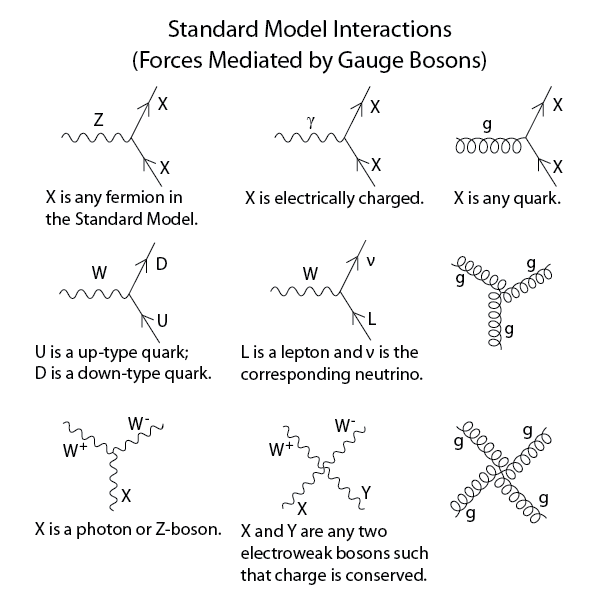
\includegraphics[width=0.75\textwidth]{Standard_Model_Feynman_Diagram_Vertices.png}
	\caption{A list of the vertices that appear in Standard Model Feynman Diagrams. Higgs Boson interactions and neutrino oscillations are omitted. Feynman rule values of the vertices are also omitted. \cite{wikipedia_SM_feynman_vertices}}
        \label{fig:SMvertices}
\end{figure}

In the SM, for processes which have longitudinally polarized W and Z bosons in the final state,
the amplitudes of the diagrams containing the Higgs Boson and of those containing TGC and QGC between electroweak bosons are separately divergent at high energies.
However, their interference between their amplitudes cancels out exactly these divergencies, maintaining the cross section finite on the whole energy spectrum.
This exact cancellation is essential to ensure the ultimate consistency of the theory, as any deviation would eventually lead to violations of the unitarity at high energies \cite{PhysRevLett.38.883}.

In the Standard Model, there are only 4 QGC allowed between electroweak bosons: $\mathrm{WWWW}$, $\mathrm{WWZZ}$, $\mathrm{WWZ\gamma}$ and $\mathrm{WW\gamma\gamma}$ (Figure \ref{fig:EWQGC}).
\begin{figure}[ht]
  \centering
  \subfigure[$\mathrm{WWWW}$]          {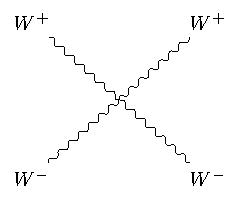
\includegraphics[width=.2\linewidth]{quartic_WWWW.pdf}}
  \subfigure[$\mathrm{WWZZ}$]          {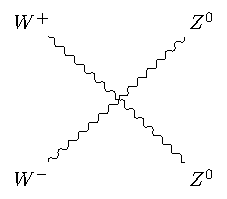
\includegraphics[width=.2\linewidth]{quartic_WWZZ.pdf}}
  \subfigure[$\mathrm{WWZ\gamma}$]     {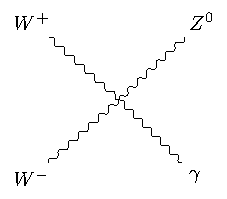
\includegraphics[width=.2\linewidth]{quartic_WWZG.pdf}}
  \subfigure[$\mathrm{WW\gamma\gamma}$]{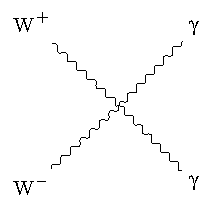
\includegraphics[width=.2\linewidth]{quartic_WWGG.pdf}}
  \caption{Electroweak Quartic Gauge Couplings allowed in the Standard Model.}
  \label{fig:EWQGC}
\end{figure}

There are several processes that are sensitive to TGCs, where their contribution is present at Leading Order (LO) in the perturbative calculations,
but for QGC they are fewer and have very small cross sections.
One of such processes is the Vector Boson Scattering (VBS).
Another process that depends on TGC and QGC at tree level is the simultaneous production of three vector bosons.

\subsection{Triboson production at LHC}
The simultaneous production of three electroweak bosons is a class of extremely rare processes that offer an interesting insight into the mechanisms of the electroweak sector of the Standard Model.
Triboson are extremely rare events which involve the simultaneous emission of three electroweak gauge bosons -- photons, W and Z bosons -- from a single hard scattering event.
The importance of these processes is due to the fact that most of them have a significant contribution from Triple Gauge Couplings (TGC) and Quartic Gauge Couplings (QGC) at Leading Order (LO).
In particular, very few processes are accessible at an hadron collider are sensitive to QGC at tree level.

A few representative Feynman diagrams for triboson production are shown in Figure \ref{fig:triboson_feynman}.
\begin{figure}[th]
  \centering
  \subfigure[]                                 {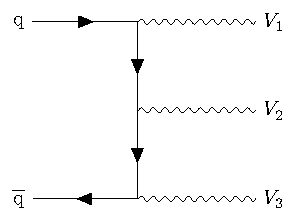
\includegraphics[width=.24\linewidth]{triboson_quarkline_VVV.pdf}}
  \subfigure[]                                 {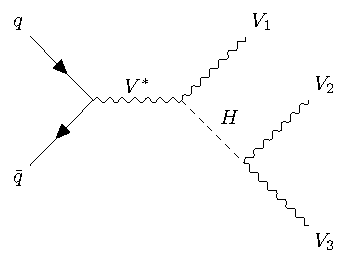
\includegraphics[width=.24\linewidth]{triboson_H_VVV.pdf}}
  \subfigure[\label{fig:triboson_feynman:TGC}] {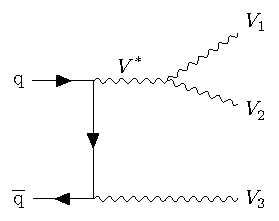
\includegraphics[width=.24\linewidth]{triboson_TGC_VVV.pdf}}
  \subfigure[\label{fig:triboson_feynman:QGC}] {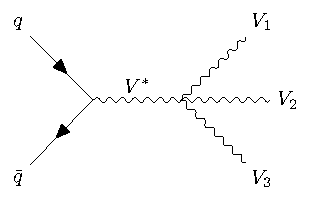
\includegraphics[width=.24\linewidth]{triboson_QGC_VVV.pdf}}
  \caption{Representative Feynman diagrams for the production of three vector bosons. Diagrams \ref{fig:triboson_feynman:TGC} and \ref{fig:triboson_feynman:QGC} are sensitive to triple and quartic gauge couplings respectively.}
  \label{fig:triboson_feynman}
\end{figure}
It must be noted that not all final states are possible through such diagrams, since electric charge must be conserved at each vertex,
the Higgs boson does not directly couple with photons and that the \PZ boson does not interact with the photon, since it is electrically neutral.
This means that no contribution from QGC (Figure \ref{fig:triboson_feynman:QGC}) is present at LO for fully neutral final states such as $\PZ\PZ\PZ$, $\PZ\PZ\PGg$, $\PZ\PGg\PGg$.

It offers the opportunity to test the predictions of the Standard Model with unparalleled precision in a complementary way with respect to the study of the Higgs Boson.

Due to the strikingly low cross section the study of these processes is extremely challenging,
although some have final states with a very low background.

\begin{table}[ht]
  \centering
  \caption{Summary of the ATLAS and CMS collaborations results on triboson production.}
  \label{tab:summary_triboson_papers}
  \renewcommand{\arraystretch}{1.5} % more space between rows in the main table
  \begin{tabular}{l l r l}
    % the nested tables use the normal spacing
    \toprule
    Experiment & Channel(s) & Energy & Significance \\
    \midrule
    ATLAS \cite{STDM-2013-05}  & $\PW\PGg\PGg$                &  8 TeV & $> 3 \sigma$                              \\ \hline
    ATLAS \cite{STDM-2014-01}  & $\PZ\PGg$, $\PZ\PGg\PGg$     &  8 TeV & $\PZ\PGg\PGg$: 6.3 $\sigma$             \\ \hline
    ATLAS \cite{STDM-2015-07}  & $\PW\PW\PW$                  &  8 TeV & 0.96 $\sigma$                             \\ \hline
    ATLAS \cite{STDM-2016-05}  & $\PW\PW\PGg$, $\PW\PZ\PGg$   &  8 TeV & $\PW\PW\PGg$ \small{(lept.)}: 1.4 $\sigma$  \\ \hline
    ATLAS \cite{STDM-2016-06}  & $\PGg\PGg\PGg$               &  8 TeV & MC overestimate                           \\ \hline
    CMS   \cite{CMS-SMP-15-008}&$\PW\PGg\PGg$, $\PZ\PGg\PGg$  &  8 TeV & \renewcommand{\arraystretch}{1.}\makecell[l]{
      $W\PGg\PGg$: 2.6 $\sigma$\\ $Z\PGg\PGg$: 5.9 $\sigma$
    } \\ \hline
    ATLAS \cite{ATLAS-STDM-2018-33}& $\PW\PGg\PGg$            & 13 TeV & 5.6 $\sigma$                              \\ \hline
    ATLAS \cite{ATLAS-STDM-2019-17}& $\PW\PZ\PGg$             & 13 TeV & 6.3 $\sigma$                              \\ \hline
    \noalign{\vspace{.3ex}}
    ATLAS \cite{STDM-2017-22}      & \makecell[l]{$\PW\PW\PW$,\\ $\PW\PW\PZ$, $\PW\PZ\PZ$} & 13 TeV & \renewcommand{\arraystretch}{1.}\makecell[l]{
      \textbf{combined}: 4.1 $\sigma$ \\ $\PW\PW\PW$ \small{(lept.+semilept.)}: 3.2 $\sigma$\\ $\PW{\rm V}\PZ$ \small{(lept.+semilept.)}: 3.2 $\sigma$
    } \\ \noalign{\vspace{.3ex}}\hline
    ATLAS \cite{HDBS-2019-16}      & $\PW\PW\PW$              & 13 TeV & 8 $\sigma$, excess over SM at 2.6 $\sigma$\\ \hline
    ATLAS \cite{STDM-2021-09}      & $\PZ\PGg\PGg$            & 13 TeV &                                           \\ \hline
    CMS   \cite{CMS-SMP-17-013}    & $\PW\PW\PW$              & 13 TeV & 0.6 $\sigma$                              \\ \hline
    \noalign{\vspace{.3ex}}
    CMS   \cite{CMS-SMP-19-014}    & \makecell[l]{$\PW\PW\PW$, $\PW\PW\PZ$,\\ $\PW\PZ\PZ$, $\PZ\PZ\PZ$} & 13 TeV & \makecell[l]{
      \textbf{combined}: 5.0 $\sigma$\\ $\PW\PW\PW$: 2.5 $\sigma$\\ $\PW\PW\PZ$: 3.5 $\sigma$\\ $\PW\PZ\PZ$: 1.6 $\sigma$\\ $\PZ\PZ\PZ$: 0 $\sigma$
    } \\ \noalign{\vspace{.3ex}}\hline
    \noalign{\vspace{.3ex}}
    CMS   \cite{CMS-SMP-19-013}    & $W\PGg\PGg$, $Z\PGg\PGg$ & 13 TeV & \renewcommand{\arraystretch}{1.}\makecell[l]{
      $W\PGg\PGg$: 3.1 $\sigma$\\ $Z\PGg\PGg$: 4.8 $\sigma$
    } \\
    \bottomrule
  \end{tabular}
\end{table}
% CMS
% SMP-15-008 & WGG, ZGG           &  8 TeV & WWG: 2.6, ZGG: 5.9                                  & http://dx.doi.org/10.1007/JHEP10(2017)072
%
% SMP-17-013 & WWW                & 13 TeV & 0.6 sigma                                           & http://dx.doi.org/10.1103/PhysRevD.100.012004
% SMP-19-014 & WWW, WWZ, WZZ, ZZZ & 13 TeV & combined: 5.0, WWW: 2.5, WWZ: 3.5, WZZ: 1.6, ZZZ: 0 & http://dx.doi.org/10.1103/PhysRevLett.125.151802
% SMP-19-013 & WGG, ZGG           & 13 TeV & WGG: 3.1, ZGG: 4.8                                  & http://dx.doi.org/10.1007/JHEP10(2021)174
%
% SMP-22-006 & WWG, HG            & 13 TeV & 5.6 sigma                                           & submitted https://cds.cern.ch/record/2875047
%
%
% ATLAS
% STDM-2013-05 & WGG           &  8 TeV & evidence, cross section & https://journals.aps.org/prl/abstract/10.1103/PhysRevLett.115.031802
% STDM-2014-01 & ZG, ZZG       &  8 TeV & 6.3 sigma               & https://journals.aps.org/prd/abstract/10.1103/PhysRevD.93.112002
% STDM-2015-07 & WWW           &  8 TeV & 0.96 sigma              & https://link.springer.com/article/10.1140/epjc/s10052-017-4692-1
% STDM-2016-05 & WWG, WZG      &  8 TeV & WWG(lept): 1.4 sigma    & https://link.springer.com/article/10.1140/epjc/s10052-017-5180-3
% STDM-2016-06 & GGG           &  8 TeV & MC overestimate         & https://www.sciencedirect.com/science/article/pii/S0370269318302533
%
% STDM-2017-22 & WWW, WWZ, WZZ & 13 TeV & & https://www.sciencedirect.com/science/article/pii/S0370269319306355
% HDBS-2019-16 & WWW           & 13 TeV & 8 sigma, excess at 2.6 sigma & https://journals.aps.org/prl/abstract/10.1103/PhysRevLett.129.061803
% STDM-2021-09 & ZGG           & 13 TeV & & https://link.springer.com/article/10.1140/epjc/s10052-023-11579-8
%
% STDM-2018-33 & WGG           & 13 TeV & & submitted https://atlas.web.cern.ch/Atlas/GROUPS/PHYSICS/PAPERS/STDM-2018-33
% STDM-2019-17 & WZG           & 13 TeV & & submitted https://atlas.web.cern.ch/Atlas/GROUPS/PHYSICS/PAPERS/STDM-2019-17

Some triboson production channels have been observed by both the ATLAS and CMS collaborations in proton-proton collisions at LHC.
The first results were obtained during \Run1 at a centre-of-mass energy of 8\TeV.

% Many articles only report a fiducial cross section, so it is more difficult to compare between experiments
% GGG
The production of three photons, $\gamma\gamma\gamma$, was observed by the ATLAS Collaboration \cite{STDM-2016-06}, with a measured cross section of $72.6 \pm 6.5 \text{(stat)} \pm 9.2 \text{(syst)}~\text{fb}$.
% WGG
Evidence for the production of $W\gamma\gamma$ was found by the ATLAS Collaboration \cite{STDM-2013-05} measuring a cross-section of $6.1^{+1.1}_{-1.0} \text{(stat)} \pm 1.2 \text{(syst)} \pm 0.2 \text{(lumi)}~\text{fb}$ for the leptonic channel,
while the CMS Collaboration \cite{CMS-SMP-15-008} measured $4.9 \pm 1.4 \text{(stat)} \pm 1.6 \text{(syst)} \pm 0.1 \text{(lumi)}~\text{fb}$.
% ZGG
Both the ATLAS \cite{STDM-2014-01} and CMS collaborations \cite{CMS-SMP-15-008} observed $Z\gamma\gamma$, measuring fiducial cross sections of
$6.2^{+1.2}_{-1.1} \text{(stat)} \pm 0.4 \text{(syst)} \pm 0.1 \text{(lumi)}~\text{fb}$ for the former,
and $12.4 \pm 1.4 \text{(stat)} \pm 1.8 \text{(syst)} \pm 0.3 \text{(lumi)}~\text{fb}$ for the latter for the leptonic decay of the Z boson.
% WWG
The ATLAS Collaboration studied the $WW\gamma$ \cite{STDM-2016-05}, measuring the inclusive cross section $\sigma(pp \rightarrow e\nu \mu\nu \gamma) = 1.5 \pm 0.9 \text{(stat)} \pm 0.5 \text{(syst)}~\text{fb}$, at 1.4 $\sigma$ level.
% WWW
Similarly, the ATLAS Collaboration set an upper limit of 730 fb \cite{STDM-2015-07} on the cross section of $W^{\pm}W^{\pm}W^{\mp}$ at 95 \% confidence level.
% by considering two decay channels, the fully leptonic $W^{\pm}W^{\pm}W^{\mp} \rightarrow \ell^{\pm} \nu \ell^{\pm} \nu \ell^{\mp} \nu$
% and the the semileptonic $W^{\pm}W^{\pm}W^{\mp} \rightarrow \ell^{\pm} \nu \ell^{\pm} \nu j j$.

In \RunII, with more data avaliable, and also the higher centre-of-mass energy of 13\TeV, more channels became accessible.
% WGG
The CMS Collaboration found evidence for $W^\pm\gamma\gamma$ \cite{CMS-SMP-19-013} and measured a fiducial cross section of
$13.6^{+1.9}_{-1.9} \text{(stat)} {}^{+4.0}_{-4.0} \text{(syst)} \pm 0.08 \text{(PDF + scale)}~\text{fb}$.
% ZGG
The ATLAS Collaboration observed $Z\gamma\gamma$ \cite{STDM-2021-09} and measured the fiducial cross section $\sigma_{Z(\rightarrow \ell\ell)\gamma\gamma} = 2.45 \pm 0.20 \text{(stat)} \pm 0.22 \text{(syst)} \pm 0.04 \text{(lumi)}~\text{fb}$,
while the CMS Collaboration found evidence for the same process \cite{CMS-SMP-19-013} and measured $5.41^{+0.58}_{-0.55} \text{(stat)} {}^{+0.64}_{-0.70} \text{(syst)} \pm 0.06 \text{(PDF + scale)}~\text{fb}$.
% VVV
The ATLAS Collaboration found evidence \cite{STDM-2017-22} and the CMS Collaboration observed \cite{CMS-SMP-19-014} the production of three massive vector bosons by combining multiple channels.
The former analysis considered $WWW$ and $WWZ$, measuring the inclusive cross sections
$\sigma_{WWW} = 0.65^{+0.16}_{-0.15} \text{(stat)} {}^{+0.16}_{-0.14} \text{(syst)}~\text{fb}$ and
$\sigma_{WWZ} = 0.55 \pm 0.14 \text{(stat)} {}^{+0.15}_{-0.13} \text{(syst)}~\text{fb}$ respectively,
finding evidence also for the two process separately.
The latter combined $WWW$, $WWZ$, $WZZ$ and $ZZZ$, measuring and inclusive cross section of $1010^{+210}_{-200}\text{(stat)}{}^{+150}_{-120}\text{(syst)}~\text{fb}$.
The individual $WWW$ and $WWZ$ channels also passed the threshold for evidence, and their cross section were measured as
$\sigma_{WWW} = 590 ^{+160}_{-150} \text{(stat)} {}^{+16}_{-130} \text{(syst)}~\text{fb}$ and
$\sigma_{WWZ} = 300 ^{+120}_{-100} \text{(stat)} {}^{+50}_{-40 } \text{(syst)}~\text{fb}$
respectively, while for $WZZ$ the significance was lower than 3 standard deviations with a measured
$\sigma_{WZZ} = 200 ^{+160}_{-110} \text{(stat)} {}^{+70}_{-20 } \text{(syst)}~\text{fb}$,
and for $ZZZ$ only an upper limit of $\sigma_{ZZZ} < 200~\text{fb}$ at 95 \% CL could be placed.
% WWW
In another paper, the ATLAS Collaboration presented the observation of $WWW$ production \cite{HDBS-2019-16},
measuring an inclusive cross-section of $820 \pm 100 \text{(stat)} \pm 80 \text{(syst)}~\text{fb}$,
with an excess approximately 2.6 standard deviations from the predicted cross section of $511 \pm 18~\text{fb}$ calculated at next-to-leading-order QCD and leading-order electroweak accuracy.

The strategy for the measurement of three yet unexplored channels of triboson production will be described in this thesis.

\section{Choice of the final state}
In this thesis a study of triboson production with two massive bosons and a photon is presented.

Vector bosons are unstable particles and, according to the Standard Model, can decay into a pair of leptons or quarks,
which build up the final state observed in the detectors.
In Table \ref{tab:VB-BR} the branching ratios (BR) of W and Z are reported.

\begin{table}
  \centering
  \caption{Branching ratios of vector bosons \cite{Workman:2022ynf}. Note: $\ell$ = e, $\mu$.}
  \label{tab:VB-BR}
  \begin{tabular}{ l r } % l -> divide intermediate and final state
    \hline
    Process & Branching ratio \\
    \hline
    $W \rightarrow e^+ \nu               $ &         (10.71 $\pm$ 0.16) \% \\
    $W \rightarrow \mu^+ \nu             $ &         (10.63 $\pm$ 0.15) \% \\
    $W \rightarrow \tau^+ \nu            $ &         (11.38 $\pm$ 0.21) \% \\
    \boldmath$W \rightarrow \ell \nu     $ & \textbf{(21.34 $\pm$ 0.22) \%}\\
    \boldmath$W \rightarrow q\bar{q}     $ & \textbf{(67.41 $\pm$ 0.27) \%}\\
    \hline
    $Z \rightarrow e^+ e^-               $ &         (3.363 $\pm$ 0.004) \% \\
    $Z \rightarrow \mu^+ \mu^-           $ &         (3.366 $\pm$ 0.007) \% \\
    $Z \rightarrow \tau^+ \tau^-         $ &         (3.370 $\pm$ 0.008) \% \\
    $Z \rightarrow \nu^+ \nu^-           $ &         (20.00 $\pm$ 0.050) \% \\
    \boldmath$Z \rightarrow \ell^+ \ell^-$ & \textbf{(6.729 $\pm$ 0.008) \%}\\
    \boldmath$Z \rightarrow q\bar{q}     $ & \textbf{(69.91 $\pm$ 0.060) \%}\\
    \hline
  \end{tabular}
\end{table}

Hadronic branching ratios are much greater than the leptonic ones: the hadronic BR for the W boson is three times the one containing at least an electron or a muon, while for Z it is 10 times larger.
Triboson production in the $\PZ\PZ\PGg$ and $\PZ\PW\PGg$ channels is an extremely rare process, as highlighted by the cross sections reported in Table \ref{tab:xsection-inclusive}.
On one hand we would like to use the decays with larger BR, but on the other hand with a clean fully leptonic final state it would be easier to separate the signal from the background.
However, the small BR (V $\rightarrow$ leptons) translates into very low production and decay cross section of $\PZ\PZ\PGg$ and $\PW\PZ\PGg$ into leptons (Table \ref{tab:xsection-exclusive}).
In addition the leptonic decay of a W boson produces a charged lepton and a neutrino, but the latter cannot be detected directly neither in CMS nor in ATLAS.
Its presence may only be deduced from the existence of an unbalance in the sum in the transverse plane of the momenta of all the particles coming from a collision,
called ``missing transverse momentum'' (\ptmiss), ``missing transverse energy'', or sometimes just ``missing energy'' (\ETmiss), abbreviated as MET.
Since the measurement of the \ptmiss is by its nature indirect, the errors associated with it are higher than for every other reconstructed entity.
As a result, searches for leptonic decays of \PW bosons suffer from the increased complexity of its reconstruction, especially in the case of two {\PW}s.
Additionally, \ptmiss is present in many different processes besides triboson production, which results in increased background.

In this analysis three channels are considered, with 4, 3, and 2 charged leptons (electrons or muons) in the final state, corresponding to
$pp \rightarrow \PZ\PZ\PGg \rightarrow 4\Pl \PGg$,
$pp \rightarrow \PW\PZ\PGg \rightarrow 3\Pl \PGn \PGg$ and
$pp \rightarrow V\PZ\PGg \rightarrow 2\Pl \PGg\ 2j$ (where $V$ is either \PZ or \PW)
respectively.

\begin{table}
  \centering
  \caption{Cross sections of triboson production and prediction of the number of events in a scenario where the integrated luminosity is 137 fb$^{-1}$.}
  \label{tab:xsection-inclusive}
  \begin{tabular}{ l c c }
    \toprule
    Process & Cross section  & \renewcommand{\arraystretch}{1.}\begin{tabular}{@{}c@{}} Events \\ $\Lumi = 137 fb^{-1}$\end{tabular} \\
    \midrule
    $\Pp\Pp \to \PZ\PZ\PGg$ & $22.02$\usep fb & $3\,016$ \\
    $\Pp\Pp \to \PW\PZ\PGg$ & $34.06$\usep fb & $4\,666$ \\
    \bottomrule
  \end{tabular}
\end{table}

\begin{table}
  \centering
  \caption{Exclusive cross sections of triboson production in the leptonic and semileptonic final states.
    Taus are excluded, meaning that $\Pl = \Pe, \PGm$.
  }
  \label{tab:xsection-exclusive}
  \begin{tabular}{ l@{}l c c } % l -> divide intermediate and final state
    \toprule
    \multicolumn{2}{c}{Process} & Branching ratio & Cross section \\ %total x BR\\
    \midrule
    $\Pp\Pp \to \PZ\PZ\PGg$ & $\to 4\Pl \PGg$      & 0.444\usep\% & 0.098\usep fb\\ % $0.\overline{4}$\usep\% & 0.09786\usep fb
    $\Pp\Pp \to \PW\PZ\PGg$ & $\to 3\Pl \PGn \PGg$ & 1.435\usep\% & 0.489\usep fb\\
    $\Pp\Pp \to \PZ\PZ\PGg$ & $\to 2\Pl \PGg\ 2j$  & 9.408\usep\% & 2.072\usep fb\\
    $\Pp\Pp \to \PW\PZ\PGg$ & $\to 2\Pl \PGg\ 2j$  & 4.536\usep\% & 1.545\usep fb\\
    \bottomrule
  \end{tabular}
\end{table}

The quarks coming from the decay of the bosons hadronize in timescales comparable to 10$^\text{-15}$ s, producing a spray of particles known as a jet.
The reconstruction and identification of such objects is explained in detail in Section \ref{sec:jets}.
The main drawback of the hadronic channels is that, in a hadron collider, jets are produced with a much higher frequency than leptons,
both as initial/final state radiation, higher order QCD corrections, and by \pileup{} events,
which translates into a much higher number of background events.
The precise reconstruction of jet properties is also more difficult, and it is not possible to distinguish the flavour of the light quark that originated a jet,
and thus separating a Z from a W becomes a very challenging task, compared to leptonic decays.

Figure \ref{fig:triboson_feynman_finalstate} shows three illustrative Feynman diagrams for each of the three channels.
It is worth noting that in the Standard Model the $\PW\PZ\PGg$ (regardless of the decay of the \PW and \PZ) production
has a leading order (perturbative expansion up to $\alpha_{EW}^6$) contribution from triple and quartic gauge couplings,
while that is not the case for $\PZ\PZ\PGg$, due to the absence of neutral TGC and QGC.

\begin{figure}[th]
  \centering
  \subfigure[] {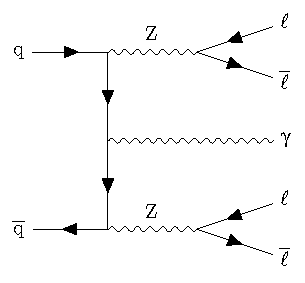
\includegraphics[width=.32\linewidth]{triboson_4LG.pdf}}
  \subfigure[] {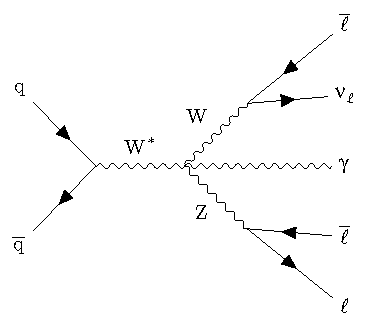
\includegraphics[width=.32\linewidth]{triboson_3LNuG.pdf}}
  \subfigure[] {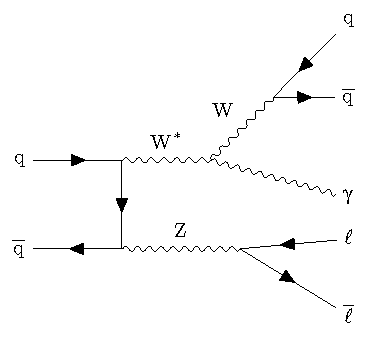
\includegraphics[width=.32\linewidth]{triboson_2L2jG.pdf}}
  \caption{Representative Feynman diagrams for the production of three vector bosons with a photon and 4, 3 or 2 charged leptons in the final state.}
  \label{fig:triboson_feynman_finalstate}
\end{figure}
